%%%%%%%%%%%%%%%%%%%%%%%%%%%%%%%%%%%%%%%%%
% Beamer Presentation
% LaTeX Template
% Version 2.0 (March 8, 2022)
%
% This template originates from:
% https://www.LaTeXTemplates.com
%
% Author:
% Vel (vel@latextemplates.com)
%
% License:
% CC BY-NC-SA 4.0 (https://creativecommons.org/licenses/by-nc-sa/4.0/)
%
%%%%%%%%%%%%%%%%%%%%%%%%%%%%%%%%%%%%%%%%%

%----------------------------------------------------------------------------------------
%	PACKAGES AND OTHER DOCUMENT CONFIGURATIONS
%----------------------------------------------------------------------------------------

\documentclass[
	11pt, % Set the default font size, options include: 8pt, 9pt, 10pt, 11pt, 12pt, 14pt, 17pt, 20pt
	%t, % Uncomment to vertically align all slide content to the top of the slide, rather than the default centered
	%aspectratio=169, % Uncomment to set the aspect ratio to a 16:9 ratio which matches the aspect ratio of 1080p and 4K screens and projectors
]{beamer}

\graphicspath{{Images/}{./}} % Specifies where to look for included images (trailing slash required)

\usepackage{booktabs} % Allows the use of \toprule, \midrule and \bottomrule for better rules in tables

%----------------------------------------------------------------------------------------
%	SELECT LAYOUT THEME
%----------------------------------------------------------------------------------------

% Beamer comes with a number of default layout themes which change the colors and layouts of slides. Below is a list of all themes available, uncomment each in turn to see what they look like.

%\usetheme{default}
%\usetheme{AnnArbor}
%\usetheme{Antibes}
%\usetheme{Bergen}
%\usetheme{Berkeley}
%\usetheme{Berlin}
%\usetheme{Boadilla}
%\usetheme{CambridgeUS}
%\usetheme{Copenhagen}
%\usetheme{Darmstadt}
%\usetheme{Dresden}
%\usetheme{Frankfurt}
%\usetheme{Goettingen}
%\usetheme{Hannover}
%\usetheme{Ilmenau}
%\usetheme{JuanLesPins}
%\usetheme{Luebeck}
\usetheme{Madrid}
%\usetheme{Malmoe}
%\usetheme{Marburg}
%\usetheme{Montpellier}
%\usetheme{PaloAlto}
%\usetheme{Pittsburgh}
%\usetheme{Rochester}
%\usetheme{Singapore}
%\usetheme{Szeged}
%\usetheme{Warsaw}

%----------------------------------------------------------------------------------------
%	SELECT COLOR THEME
%----------------------------------------------------------------------------------------

% Beamer comes with a number of color themes that can be applied to any layout theme to change its colors. Uncomment each of these in turn to see how they change the colors of your selected layout theme.

%\usecolortheme{albatross}
%\usecolortheme{beaver}
%\usecolortheme{beetle}
%\usecolortheme{crane}
%\usecolortheme{dolphin}
%\usecolortheme{dove}
%\usecolortheme{fly}
%\usecolortheme{lily}
%\usecolortheme{monarca}
%\usecolortheme{seagull}
%\usecolortheme{seahorse}
%\usecolortheme{spruce}
%\usecolortheme{whale}
%\usecolortheme{wolverine}

%----------------------------------------------------------------------------------------
%	SELECT FONT THEME & FONTS
%----------------------------------------------------------------------------------------

% Beamer comes with several font themes to easily change the fonts used in various parts of the presentation. Review the comments beside each one to decide if you would like to use it. Note that additional options can be specified for several of these font themes, consult the beamer documentation for more information.

\usefonttheme{default} % Typeset using the default sans serif font
%\usefonttheme{serif} % Typeset using the default serif font (make sure a sans font isn't being set as the default font if you use this option!)
%\usefonttheme{structurebold} % Typeset important structure text (titles, headlines, footlines, sidebar, etc) in bold
%\usefonttheme{structureitalicserif} % Typeset important structure text (titles, headlines, footlines, sidebar, etc) in italic serif
%\usefonttheme{structuresmallcapsserif} % Typeset important structure text (titles, headlines, footlines, sidebar, etc) in small caps serif

%------------------------------------------------

%\usepackage{mathptmx} % Use the Times font for serif text
\usepackage{palatino} % Use the Palatino font for serif text

%\usepackage{helvet} % Use the Helvetica font for sans serif text
\usepackage[default]{opensans} % Use the Open Sans font for sans serif text
%\usepackage[default]{FiraSans} % Use the Fira Sans font for sans serif text
%\usepackage[default]{lato} % Use the Lato font for sans serif text

%----------------------------------------------------------------------------------------
%	SELECT INNER THEME
%----------------------------------------------------------------------------------------

% Inner themes change the styling of internal slide elements, for example: bullet points, blocks, bibliography entries, title pages, theorems, etc. Uncomment each theme in turn to see what changes it makes to your presentation.

%\useinnertheme{default}
\useinnertheme{circles}
%\useinnertheme{rectangles}
%\useinnertheme{rounded}
%\useinnertheme{inmargin}

%----------------------------------------------------------------------------------------
%	SELECT OUTER THEME
%----------------------------------------------------------------------------------------

% Outer themes change the overall layout of slides, such as: header and footer lines, sidebars and slide titles. Uncomment each theme in turn to see what changes it makes to your presentation.

%\useoutertheme{default}
%\useoutertheme{infolines}
%\useoutertheme{miniframes}
%\useoutertheme{smoothbars}
%\useoutertheme{sidebar}
%\useoutertheme{split}
%\useoutertheme{shadow}
%\useoutertheme{tree}
%\useoutertheme{smoothtree}

%\setbeamertemplate{footline} % Uncomment this line to remove the footer line in all slides
%\setbeamertemplate{footline}[page number] % Uncomment this line to replace the footer line in all slides with a simple slide count

%\setbeamertemplate{navigation symbols}{} % Uncomment this line to remove the navigation symbols from the bottom of all slides

%----------------------------------------------------------------------------------------
%	PRESENTATION INFORMATION
%----------------------------------------------------------------------------------------

\title[HERACLES]{HERACLES: Hyperbolic Embeddings for Reconstruction and Analysis of Lineages} % The short title in the optional parameter appears at the bottom of every slide, the full title in the main parameter is only on the title page


\author[Gilad Turok]{Gilad Turok} % Presenter name(s), the optional parameter can contain a shortened version to appear on the bottom of every slide, while the main parameter will appear on the title slide

\institute[]{Columbia University, Pe'er Lab \\ \smallskip Supervised by Sitara Persad} % Your institution, the optional parameter can be used for the institution shorthand and will appear on the bottom of every slide after author names, while the required parameter is used on the title slide and can include your email address or additional information on separate lines

\date[\today]{Semester Report \\ \today} % Presentation date or conference/meeting name, the optional parameter can contain a shortened version to appear on the bottom of every slide, while the required parameter value is output to the title slide

%----------------------------------------------------------------------------------------

\begin{document}

%----------------------------------------------------------------------------------------
%	TITLE SLIDE
%----------------------------------------------------------------------------------------

\begin{frame}
	\titlepage % Output the title slide, automatically created using the text entered in the PRESENTATION INFORMATION block above
\end{frame}

%----------------------------------------------------------------------------------------
%	TABLE OF CONTENTS SLIDE
%----------------------------------------------------------------------------------------

% The table of contents outputs the sections and subsections that appear in your presentation, specified with the standard \section and \subsection commands. You may either display all sections and subsections on one slide with \tableofcontents, or display each section at a time on subsequent slides with \tableofcontents[pausesections]. The latter is useful if you want to step through each section and mention what you will discuss.

\begin{frame}
	\frametitle{Outline} % Slide title, remove this command for no title
	
	\tableofcontents % Output the table of contents (all sections on one slide)
	%\tableofcontents[pausesections] % Output the table of contents (break sections up across separate slides)
\end{frame}

%----------------------------------------------------------------------------------------
%	PRESENTATION BODY SLIDES
%----------------------------------------------------------------------------------------

%----------------------------------------------------------------------------------------
\section{Background}
%----------------------------------------------------------------------------------------

%------------------------------------------------

\begin{frame}
	\frametitle{Background: Phylogeny}

	\begin{itemize}
		\item \textbf{Phylogeny:} evolutionary development and diversification
		
		\item \textbf{Phylogenetic Tree:}
		\begin{figure}
			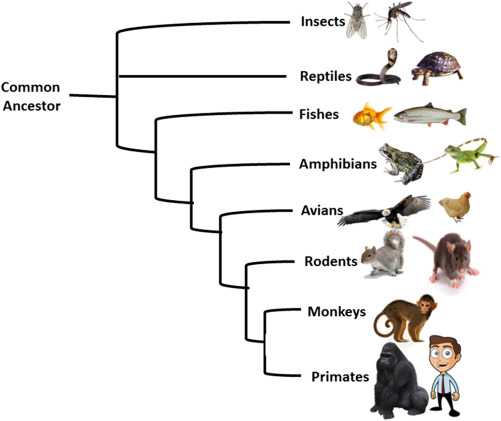
\includegraphics[width=0.5\linewidth]{phylogeny-background.jpeg}
		\end{figure}

		\item \textbf{Idea:} Use inherited genetic alterations to infer phylogenetic trees

	\end{itemize}

\end{frame}

%------------------------------------------------

\begin{frame}
	\frametitle{Background: CRISPR/Cas9}

	\begin{itemize}
		\item Use CRISPR-Cas9 to precisely insert or delete genes in a cell at specific \emph{target sites}
		\item These alterations will propogate through cell as they evolve
		\item In "leaf cells", examine the genes at target sites to reconstruct the cell lineage
	\end{itemize}

\end{frame}

%------------------------------------------------

\begin{frame}
	\frametitle{Background: Character Matrix}

	\begin{figure}
		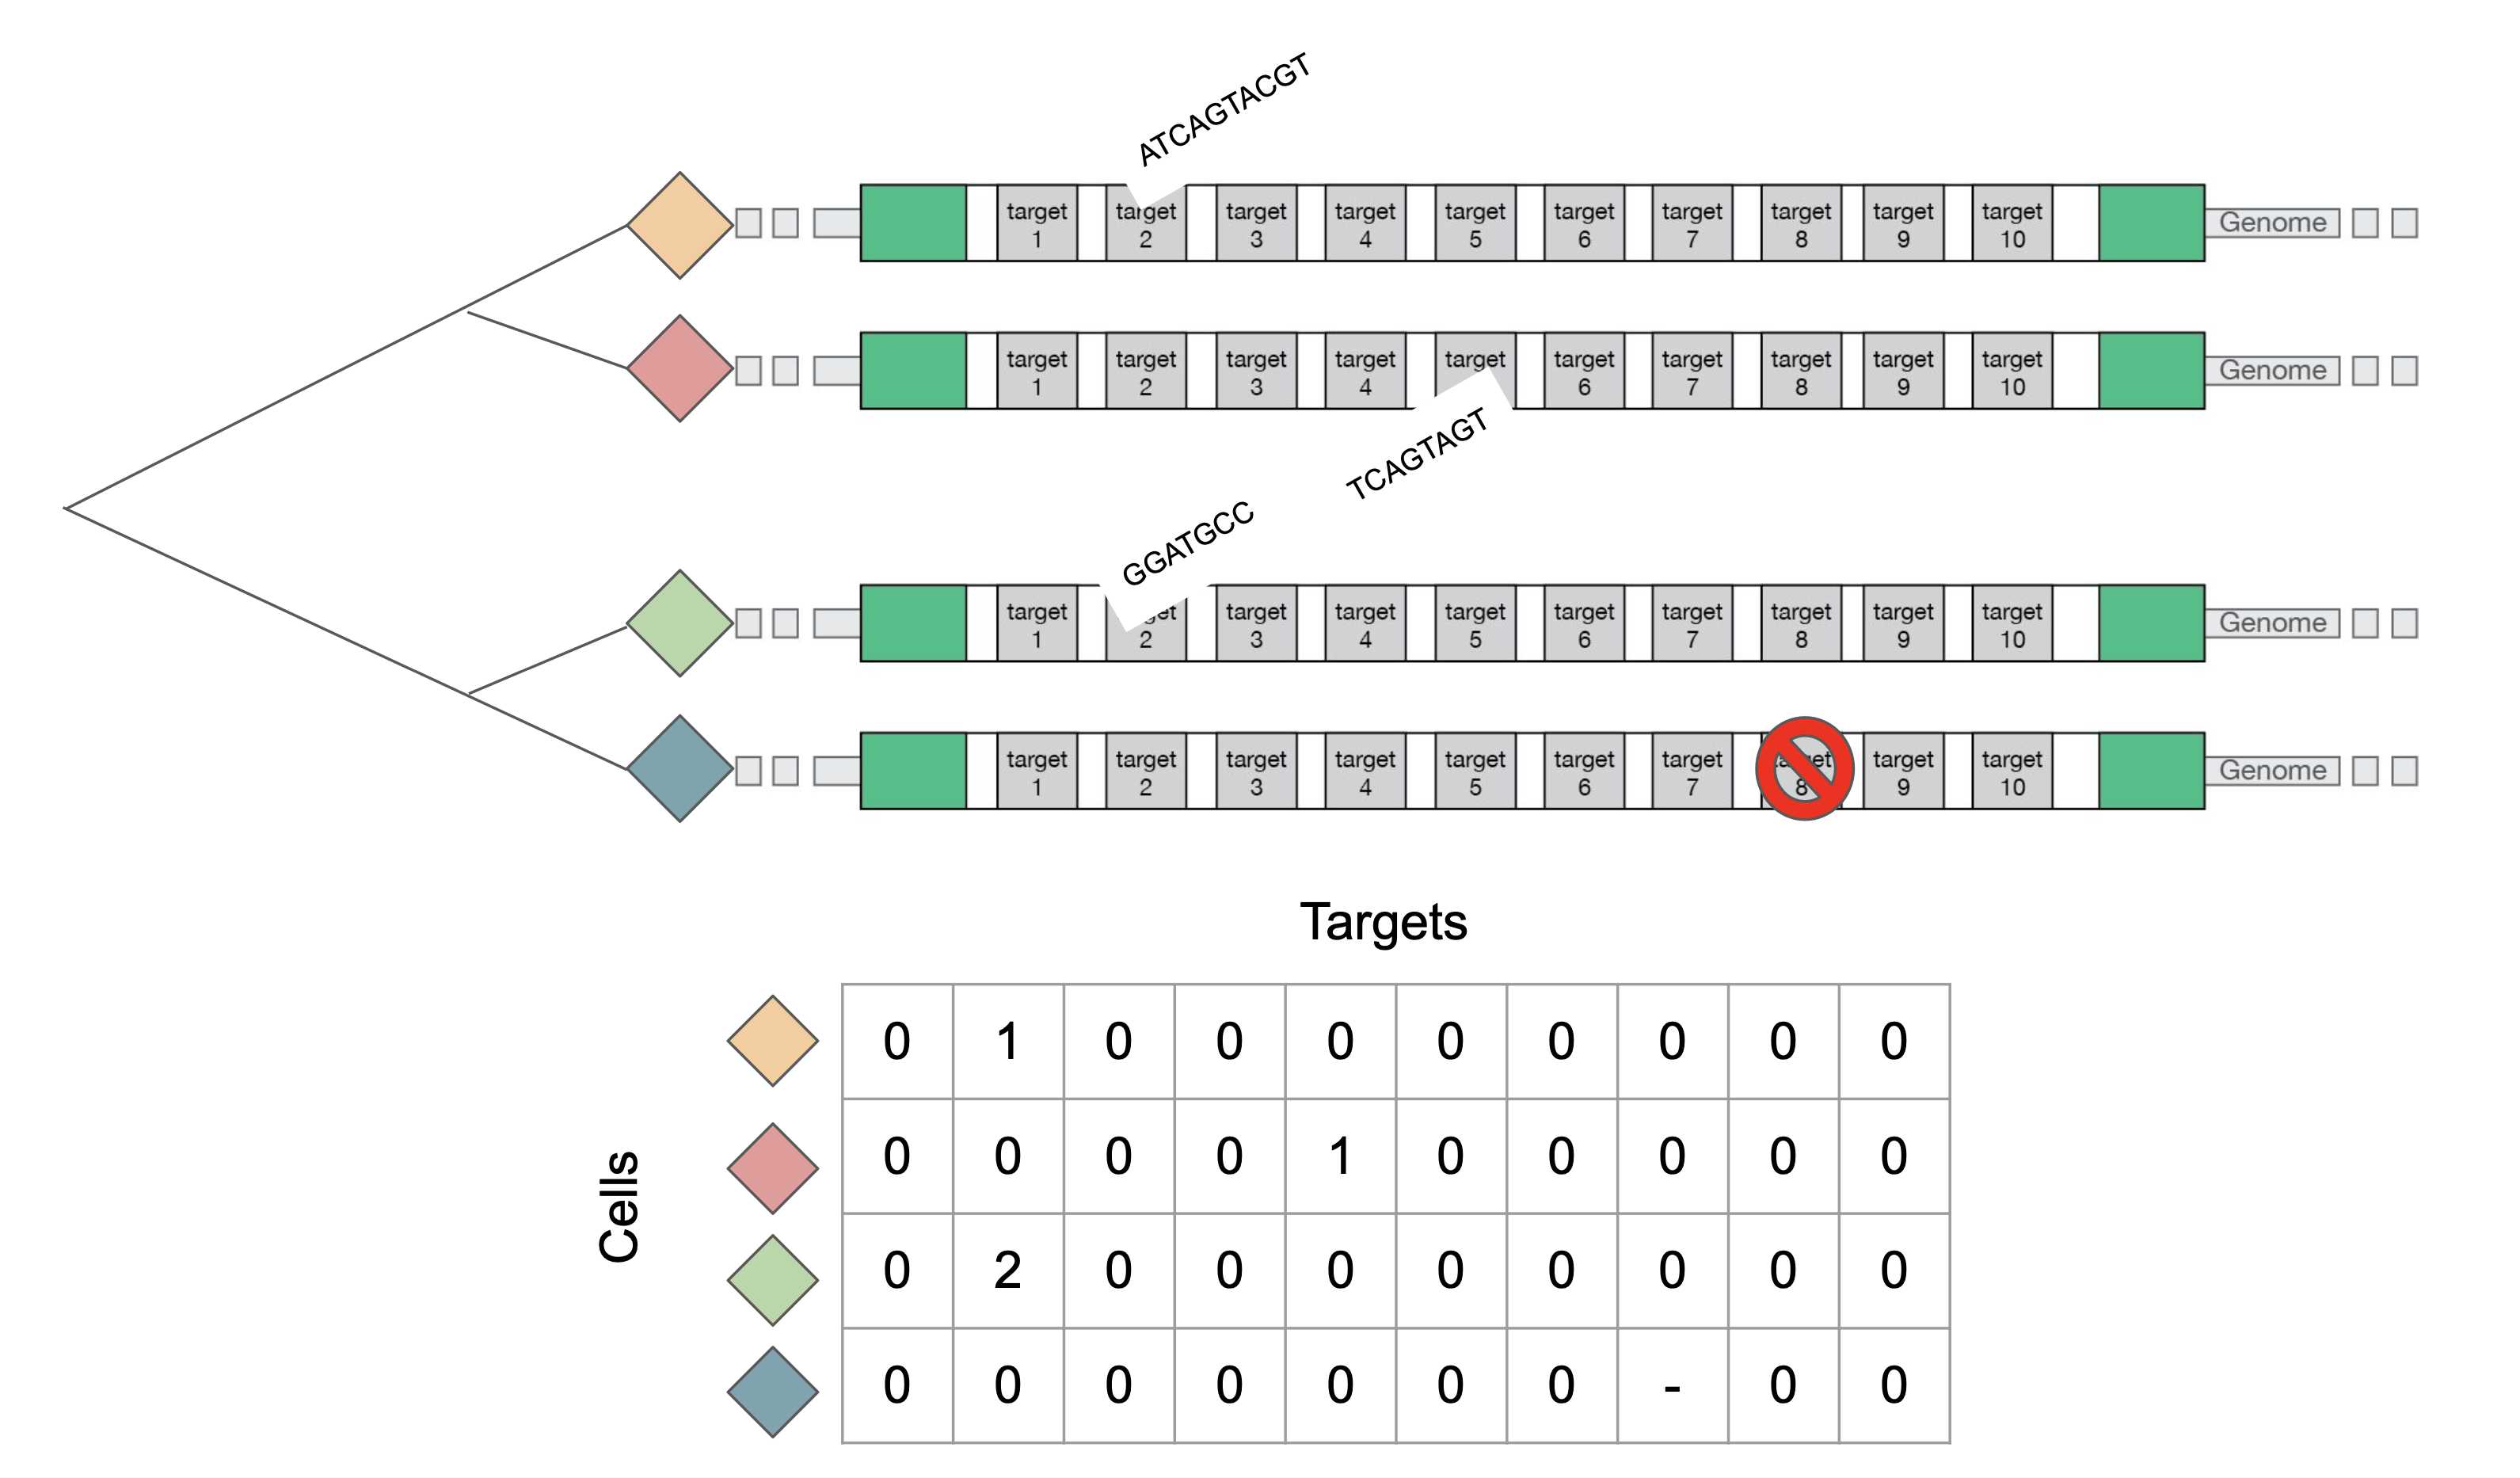
\includegraphics[width=0.95\linewidth]{anthony.png}
	\end{figure}

	Figure from Anthony's presentation
\end{frame}

%----------------------------------------------------------------------------------------
\section{Related Work}
%----------------------------------------------------------------------------------------

\begin{frame}
	\frametitle{Related Work: Methods for Lineage Tracing}

	\textbf{Distance-Based Methods:}
	\begin{itemize}
		\item Define pairwise distance function for two cells $d(c_1, c_2)$ that captures how "far away" their sequences are
		\item Learn all-to-all distance matrix based $D$ on $d$
		\item Construct tree from distance matrix $D$
	\end{itemize}

	\pause

	\textbf{Maximum Likelihood:}
	\begin{itemize}
		\item Assume statistical model of DNA sequence evolution
		\item Infer probability distribution for diffirerent configigurations of phylogenetic trees
		\item Optimize over continous branch lengths and \emph{discrete} tree topologies
	\end{itemize}

	\pause

	\textbf{Maximum Parsimony:} identify phylogenetic tree with smallest number of evolutionary events to explain sequence data

	\textbf{Bayesian Inference:} similar to maximum likelihood, but with Bayesian priors
\end{frame}

%------------------------------------------------

\begin{frame}
	\frametitle{Related Work: Wilson Paper}

	\begin{itemize}
		\item \textbf{Paper:} \textit{Learning Phylogenetic Trees as Hyperbolic Point Configurations} by Benjamin Wilson, 2021  
		\item \textbf{Idea:} \emph{Distance-based methods} in hyperbolic space can approximate \emph{maximum likelihood methods}
		\item \textbf{Motivation:} Can embed a tree into hyperbolic space with an error bounded by $2\delta$
		
		\begin{theorem}[Relaxed $4$ Point Condition]
			Let $\delta \geq 0$. A metric space $(X, d)$ is said to be $\delta$-hyperbolic if, for all $w,x,y,z \in X$,
			\begin{equation*}
				d(x,w) + d(y,z) \leq \max \big\{d(x,y) + d(z,w), \; d(x,z) + d(y,w) \big\} + 2 \delta
			\end{equation*}
		\end{theorem}

	\end{itemize}
\end{frame}

%------------------------------------------------

\begin{frame}
	\frametitle{Related Work: Wilson Paper}

	\begin{columns}[t]
		\begin{column}{0.50\textwidth}
			\begin{figure}
				
\includegraphics[width=0.8\linewidth]{euclidean-tree.png}
				\caption{Euclidean Tree-Embedding}
			\end{figure}
		\end{column}

		\begin{column}{0.50\textwidth}
			\begin{figure}
				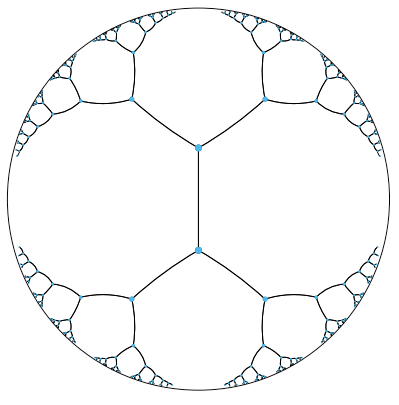
\includegraphics[width=0.8\linewidth]{hyperbolic-tree.png}
				\caption{Hyperbolic Tree-Embedding}
			\end{figure}
		\end{column}
	\end{columns}

\end{frame}

%------------------------------------------------

\begin{frame}
	\frametitle{Related Work: Wilson Paper}

	For a Riemannian manifold $M=\mathbb{R}^m$, let a point configuration $\mathbf{x}=x_1 \ldots x_n \in M$ with distance function $d$

	\bigskip

	For $N$ cells and sequence data $\Theta$ of length $L$, let $\mathcal{L}_{ij}(t \mid \Theta)$ represent the likelihood of an evolutionary distance of $t$ between cells $i,j$ given sequence data $\Theta$

	\pause

	\bigskip

	Our objective \emph{logalike} function is
	\begin{equation*}
		\mathbf{l}(\mathbf{x})=\frac{1}{L} \sum_{i \neq j} \log \mathcal{L}_{ij}(d(x^i, x^j) \mid \Theta)
	\end{equation*}
	\pause 

	Unlike typical log-likelihood on treespace, $\mathbf{l}(\mathbf{x})$ is on a Riemannian manifold and is differentiable in $\mathbf{x}$
	\bigskip
	
	Can compute $\nabla_{x^i} \mathbf{l}(x^i)$ to learn ideal point configuration for infering phylogenetic tree
\end{frame}

%------------------------------------------------

\begin{frame}
	\frametitle{Related Work: Wilson Paper}

	Let $\sigma_i$ be the base/state at target site $\sigma$ for cell $i$
	\bigskip

	Assume evolution is a continous time markov chain with transition probablities $P$, infinitesmial generator $Q$, and stationary distribution $\pi$.
	\bigskip
	
	Specifically let $P_{\sigma_i \sigma_j}(t)$ represent the probability of observing state $\sigma_j$ $t$ time steps after observing state $\sigma_i$ under the Jukes-Cantor model of mutation:

	\begin{columns}[t]
		\begin{column}{0.70\textwidth}
			\begin{equation*}
				P_{ab} = 
					\begin{cases}
						\frac{1}{4} + \frac{3}{4} e^{-4t/3} := P_{\textrm{diag}} & \textrm{if } a=b \\
						\frac{1}{4} - \frac{1}{4} e^{-4t/3} := P_{\setminus \textrm{diag}} & \textrm{otherwise}
					\end{cases}
			\end{equation*}

			\bigskip
			Figure from Sitara
		\end{column}

		\begin{column}{0.30\textwidth}
			\begin{figure}
				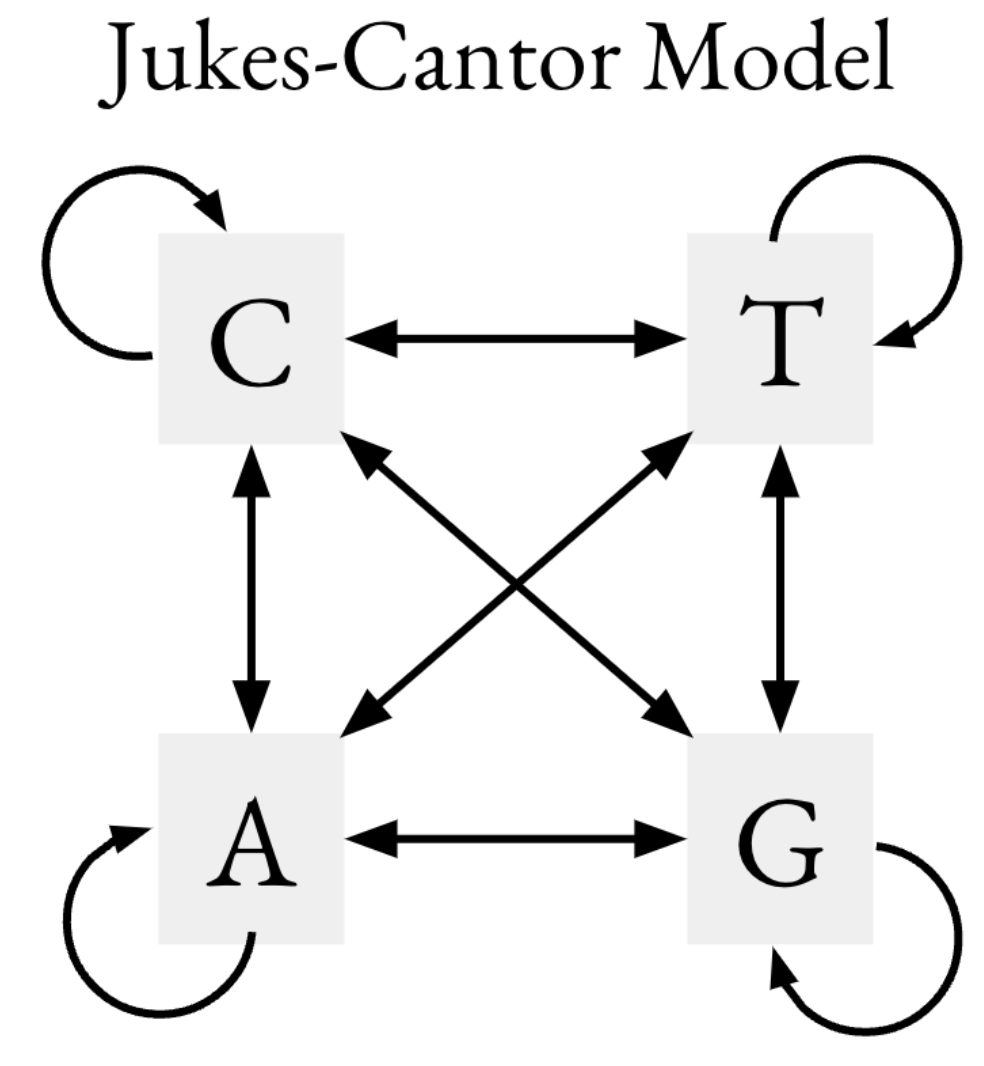
\includegraphics[width=0.8\linewidth]{jukes-cantor.png}
			\end{figure}
		\end{column}
	\end{columns}
\end{frame}

%------------------------------------------------

\begin{frame}
	\frametitle{Related Work: Wilson Paper}
	Objective logalike function:
	\begin{align*}
		\mathbf{l}(\mathbf{x} )&= \frac{1}{L} \sum_{i \neq j} \log \mathcal{L}_{ij}(d(x^i, x^j) \mid \Theta) \\
	\end{align*}
	Likelihood under assumed model of mutation
	\begin{align*}
		\mathcal{L}_{ij}(t) &= \prod_{\textrm{sites } \sigma} \pi_{\sigma_i} P_{\sigma_i \sigma_j}(t) \\
		\log \mathcal{L}_{ij}(t) &= \sum _{\textrm{sites } \sigma} \log  P_{\sigma_i \sigma_j}(t) + C \\
	\end{align*}
	Expression for gradient with respect to cell $i$
	\begin{align*}
		\nabla_{x^i} \mathbf{l}(x^i) &= \frac{1}{L} \sum_{\textrm{cells } j} \sum_{\textrm{sites } \sigma} \frac{(QP(d_{ij}))_{\sigma_i, \sigma_j}}{P(d_{ij})_{\sigma_i \sigma_j}} \nabla_{x^i} d_{x^j}
	\end{align*}
\end{frame}

%----------------------------------------------------------------------------------------
\section{HERACLES Method}
%----------------------------------------------------------------------------------------

\begin{frame}
	\frametitle{HERACLES Method: Model of Mutation}
	Accumulation of CRISPR-Cas9 mutations evolves as a continous time Markov Chain
	\bigskip

	Use a different model of mutation because known ancestral state, mutations cannot be undone, etc
	
	\begin{figure}
		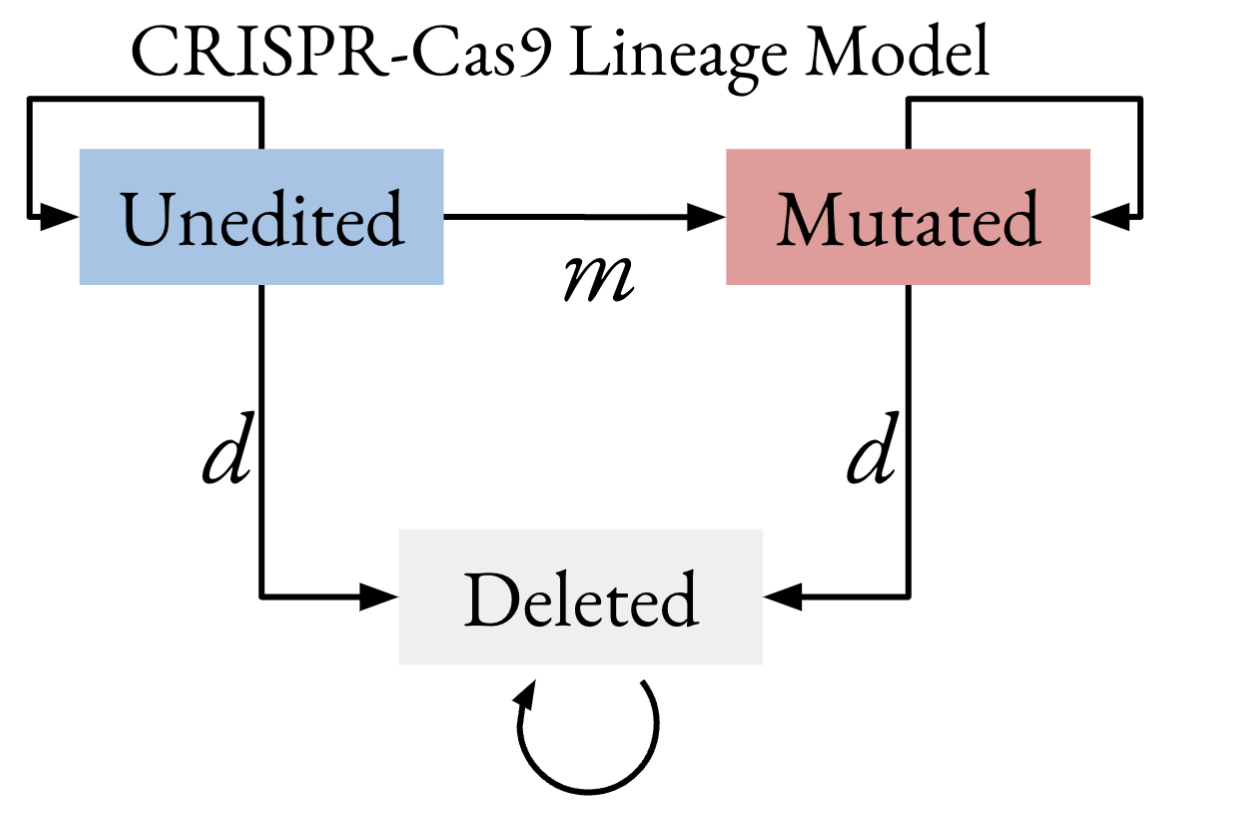
\includegraphics[width=0.55 \linewidth]{crispr-lineage-model.png}
	\end{figure}
	Figure from Sitara
\end{frame}

%------------------------------------------------

\begin{frame}
	\frametitle{HERACLES Method}

	For a cell $c$ at site $\sigma$, possible mutation states are unedited $\phi_c$, mutations $1 \ldots M_\sigma$, or deleted $D$:

	\begin{equation*}
		\sigma_c \in \{\phi_c, 1, 2 \ldots M_\sigma, D \}
	\end{equation*}

	For mutation states $a,b$, let $P_{ab}^\sigma (t)$ be the conditional probability of observing state $b$ after $t$ time units have passed since observing state $a$.
\end{frame}

%------------------------------------------------

\begin{frame}
	\frametitle{HERACLES Method}
	Because of time-irrervsersibility, distance betwen cells $i,j$ at site $\sigma$ is determined by distance from common ancestor to each cell.
	\bigskip

	Let $A(\sigma_i, \sigma_j)$ be the set of all possible ancestors of cells $i,j$ at site $\sigma$. Let $\pi_a$ be the prior of observing ancestral state $a \in A$

	\begin{align*}
		\mathcal{L}_{ij}(t) = \prod_{\textrm{sites } \sigma} \sum_{a \in A(\sigma_i, \sigma_j)} \pi_a \; P_{a \sigma_i}(\frac{t}{2}) \; P_{a \sigma_j}(\frac{t}{2})
	\end{align*}

	Biological constraints ensure set of ancestral states is small
\end{frame}

%------------------------------------------------

\begin{frame}
	\frametitle{HERACLES Method}

	The infinitesmial generator  $Q$ is defined below
	\bigskip
	
	The time to leave the unedited state and transition to a mutated or deleted state follows an exponential distribution with rate $\gamma = \gamma_M + \gamma_D$
	\bigskip
	
	Given that a transition occurs to another character state, the transition to the observed character state $C$ is $p_{\phi_\sigma, c}$
	\bigskip

	After transitioning to a character state, it may transition to a deleted state with rate $\lambda_D$
\end{frame}

%------------------------------------------------

\begin{frame}
	\frametitle{HERACLES Method}
	Infentiesmal generator $Q$ is defined below with $\sum_i P_{\phi i} = 1$

	\begin{figure}
		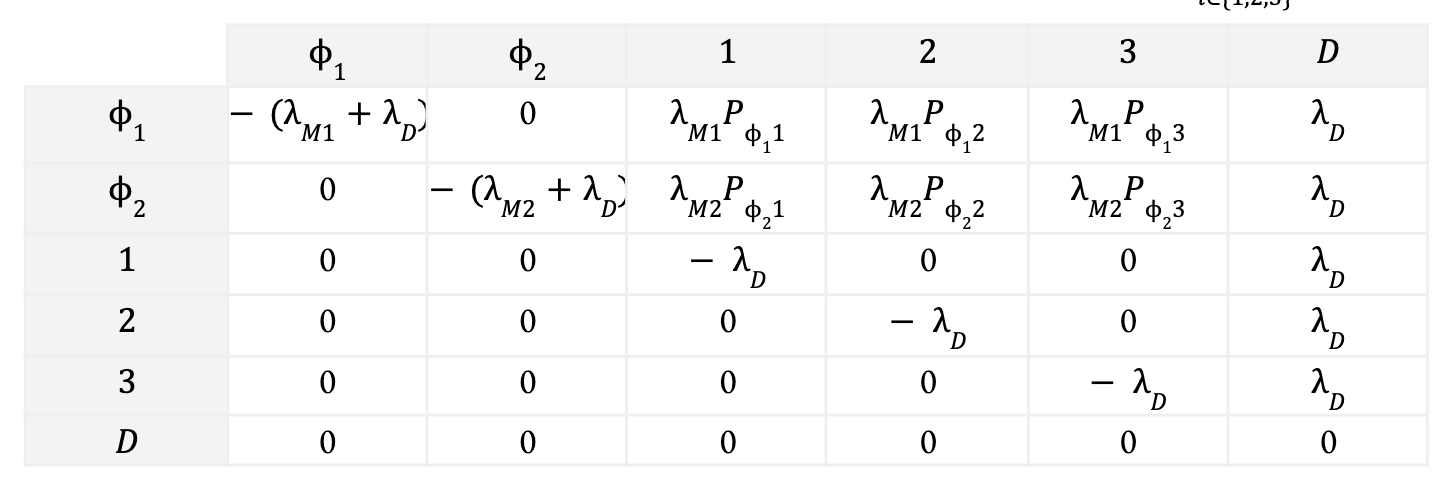
\includegraphics[width=0.95 \linewidth]{rate-matrix-q.png}
	\end{figure}

	Probability transition matrix $P$ is derived from $Q$:

	\begin{equation*}
		P(t) = \textrm{expm}(Q * t)
	\end{equation*}
\end{frame}

%------------------------------------------------

\begin{frame}
	\frametitle{HERACLES Method}
	Objective logalike function:
	\begin{align*}
		\mathbf{l}(\mathbf{x} )&= \frac{1}{L} \sum_{i \neq j} \log \mathcal{L}_{ij}(d(x^i, x^j) \mid \Theta) \\
	\end{align*}
	Likelihood under assumed model of mutation
	\begin{align*}
		\mathcal{L}_{ij}(t) &= \prod_{\textrm{sites } \sigma} \sum_{a \in A(\sigma_i, \sigma_j)} \pi_a \; P_{a \sigma_i}(\frac{t}{2}) \; P_{a \sigma_j}(\frac{t}{2}) \\
		\log \mathcal{L}_{ij}(t) &= \sum _{\textrm{sites } \sigma} \log \sum_{a \in A(\sigma_i, \sigma_j)} \pi_a \; P_{a \sigma_i}(\frac{t}{2}) \; P_{a \sigma_j}(\frac{t}{2}) \\
	\end{align*}
	Expression for gradient with respect to cell $i$
	\begin{align*}
		\nabla_{x^i} \mathbf{l}(x^i) &= \frac{1}{L} \sum_{\textrm{cells } j} \sum_{\textrm{sites } \sigma} \frac{(QP(d_{ij}))_{\sigma_i, \sigma_j}}{P(d_{ij})_{\sigma_i \sigma_j}} \nabla_{x^i} d_{x^j}
	\end{align*}
\end{frame}

%------------------------------------------------

\begin{frame}
	\frametitle{HERACLES Method}

	Focused on implementing Riemannian SGD
	\begin{figure}
		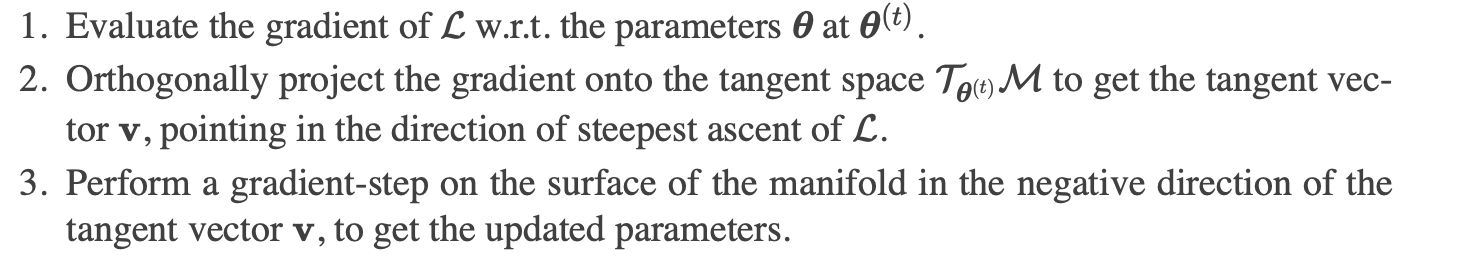
\includegraphics[width=0.9 \linewidth]{riemmanian-sgd.png}
	\end{figure}
	\pause
	Already have gradient in closed form

	\begin{figure}
		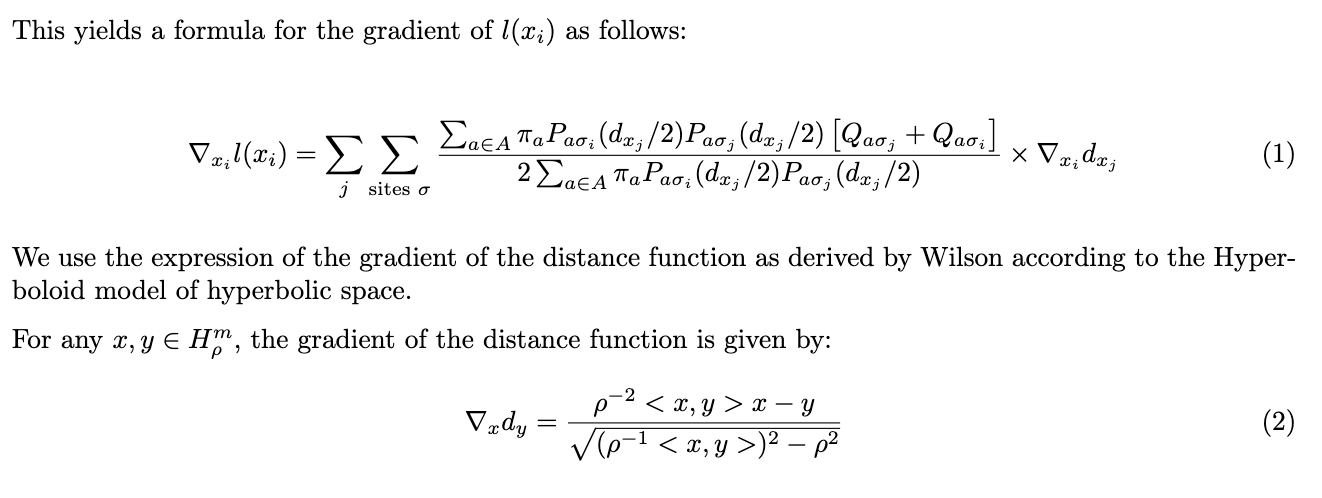
\includegraphics[width=0.8 \linewidth]{gradient.png}
	\end{figure}
\end{frame}

%------------------------------------------------

\begin{frame}
	\frametitle{HERACLES Method}
	Use automatic differentiation to simplify implementation
	\bigskip

	Use geoopt package that extends PyTorch to work with Riemannian manifolds

	\begin{figure}
		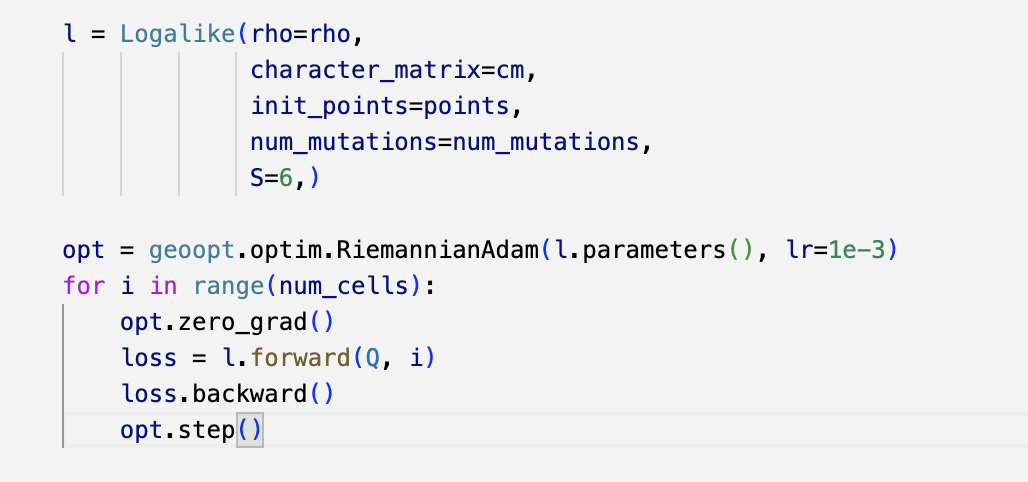
\includegraphics[width=0.8 \linewidth]{training-code.png}
	\end{figure}
\end{frame}

%------------------------------------------------

\begin{frame}
	\frametitle{HERACLES Method}

	Currently finishing implementation

	\begin{itemize}
		\item Compute prior ancestral states $\pi_a$
		\item Update simulated data with Caissopea package
		\item Extract rate variables for infentiesmal generator $Q$
	\end{itemize}
\end{frame}

\section{Conclusion}

%----------------------------------------------------------------------------------------
%	ACKNOWLEDGMENTS SLIDE
%----------------------------------------------------------------------------------------

\begin{frame}
	\frametitle{Acknowledgements}
	
	Massive thank you to Sitara and Prof Pe'er for guidance.
	\bigskip

	(And thanks to Anthony for his prior work and walking me through his code)
\end{frame}

\end{document} 